% \section{Event-driven Burst Buffer Simulator}
% \label{Sec:Simulation}

% We develop an event-driven simulator for burst buffer enabled HPC system, named \textbf{BBSim},
% from scratch in Python to mimic Cerberus scheduling Trinity.\NOTE{Fig has no info about Trinity}
% It roughly consists of 1,400 lines of code.
% Figure~\ref{Fig:JobFSM} illustrates the simulation lifetime of a job in BBSim
% using extended finite state machine (EFSM).
% The \textit{state} of the job changes depending on current status and
% happening \textit{events}, along with which an \textit{action} is taken.
% For example, at the very beginning, submitted $job_i$ will enter \textbf{Waiting Stage-in} state;
% at the meanwhile, $job_i$ is enqueued to $Q_I$ and scheduler is triggered to do scheduling.

%=========XY===========
\section{BBSim: An Event Driven Simulator of Cerberus}
\label{Sec:Simulation}

We develop an event-driven simulator, named \textbf{BBSim},
to simulate how Cerberus schedules jobs on burst-buffer-enabled HPC systems.
Besides demonstrating the lifetime of a job scheduled by Cerberus,
Figure~\ref{Fig:JobFSM} also illustrates the various events in BBSim and how to handle
them in an event-driven-simulation approach.
The changes of job \textit{state} depend on the current status and the \textit{events} to trigger \textit{actions}.
For example, when $job_i$ is submitted to the system,
it enters the \textit{Waiting Stage-in} state,
waiting to be scheduled in the job queue $Q_I$. 
The scheduler checks $job_i$'s resource demand and
dispatches it to run when sufficient resources are available.

% Whenever job enters one of its 3 phases, system resources are allocated:
% \begin{itemize}
%         \item $BB_{in}$ TB amount of burst buffer are allocated upon entering stage-in phase.
%         \item $CN$ number of compute nodes and $BB_{run}$ amount of burst buffer
%                 are allocated upon entering running phase.
%         \item $BB_{out}$ TB of burst buffer are allocated upon entering stage-out phase.
% \end{itemize}
% Various \texttt{release()} actions are of importance because, in addition to submission,
% \texttt{schedule()} is invoked to schedule waiting jobs
% whenever system resources are released:
% \begin{itemize}
%         \item When job's data is loaded from burst buffer to memory,
%                 burst buffer allocated at stage-in phase are released.
%         \item When job finishes running, system reclaims burst buffer nodes
%                 used for checkpointing.
%         \item When job's data is written to burst buffer from memory,
%                 compute nodes taken by job are returned.
%         \item When job's data is staged out to external disk,
%                 its burst buffer nodes are released.
% \end{itemize}
% 
% \begin{figure}[!t]
% \centering
%         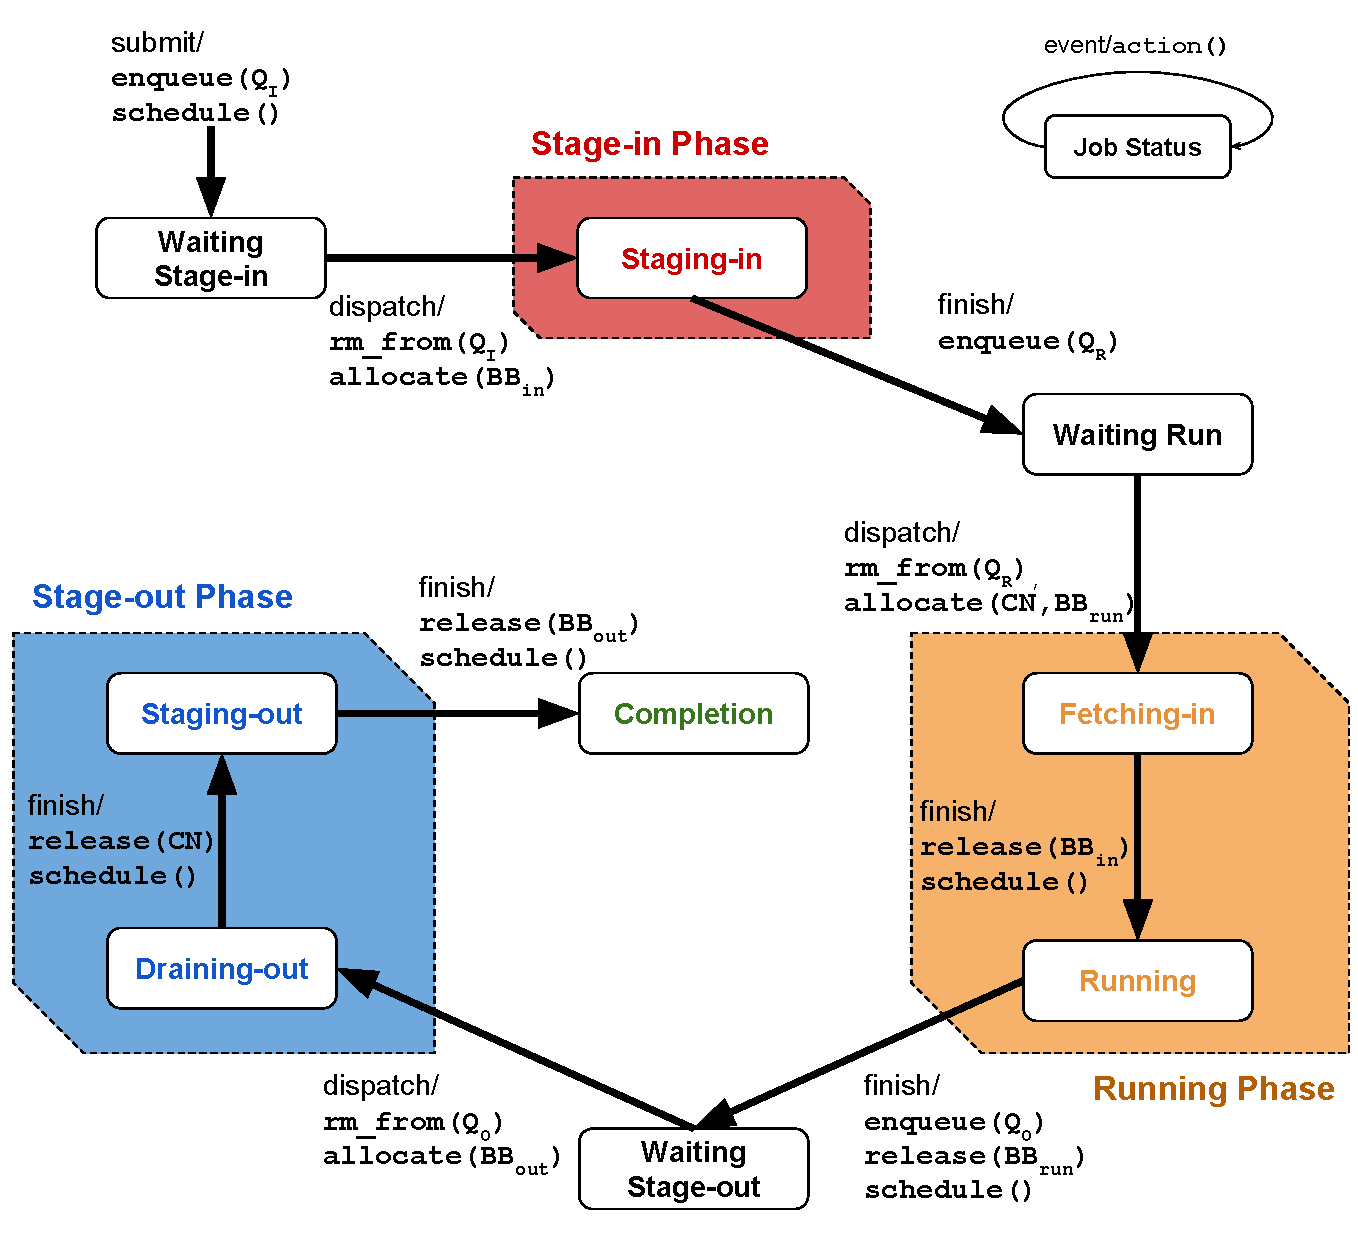
\includegraphics[width=3.6in]{3PhaseJobFSM}
%         \caption{Finite State Machine of Scheduling Simulation}
% \label{Fig:JobFSM}
% \end{figure}


%Whenever $job_i$ enters one of the three phases, the system resources are allocated in the following way:
%\begin{itemize}
        %\item $BB_{in}$ TB amount of burst buffer are allocated upon entering the stage-in phase.
        %\item $CN$ number of compute nodes and $BB_{run}$ amount of burst buffer
                %are allocated upon entering the running phase.
        %\item $BB_{out}$ TB of burst buffer is allocated upon entering the stage-out phase.
%\end{itemize}

Various \texttt{release()} actions are important because, in addition to job submissions,
\texttt{schedule()} is invoked to schedule the waiting jobs.
The allocated resource can only be released when one phase is finished.
Therefore, any \textit{dispatch} event, generated by the \texttt{schedule()} action,
follows a certain \textit{finish} event.
The allocated resources are released at the following time points:
\begin{itemize}
        \item When $job_i$ pre-fetches data from the burst buffer to the memory,
                the burst buffer allocated in the stage-in phase ($BB_{in}$) is released.
        \item When $job_i$ completes the computation,
                the system reclaims the burst buffer allocated in the running phase ($BB_{run}$).
        \item When $job_i$ output data is written to the burst buffer from the memory,
              compute nodes ($CN$) allocated in the running phase are released.
        \item When output data are drained out to the external storage,
                the burst buffer allocated in the stage-out phase ($BB_{out}$) is released.
                The simulation for $job_i$ completes.
\end{itemize}




% Notice that resource can only be released when certain phase is finished.
% Therefore, any \textit{dispatch} event, caused by \texttt{schedule()} action, actually happens
% at the meanwhile of a certain \textit{finish} event.
% The timestamps of all possible \textit{finish} events are calculated in the following way:
% \begin{align}
%         & TS_{f\_stagein} = TS_{s\_stagein} + \frac{bb\_in}{BW_{io\_to\_bb}}\label{Equ:FinIn} \\
%         & TS_{f\_loadin} = TS_{s\_run} + \frac{bb\_in}{BW_{bb\_to\_cn}}\label{Equ:FinMemIn} \\
%         & TS_{f\_run} = TS_{f\_loadin} + \frac{bb\_run}{BW_{cn\_to\_bb}} + rt\label{Equ:FinRun} \\
%         & TS_{f\_loadout} = TS_{s\_stageout} + \frac{bb\_out}{BW_{cn\_to\_bb}}\label{Equ:FinMemOut} \\
%         & TS_{f\_stageout} = TS_{f\_loadout} + \frac{bb\_out}{BW_{bb\_to\_io}} \label{Equ:FinOut}
% \end{align}
% where $TS_{f\_x}$ stands for the timestamps of finishing phase $x$,
% $TS_{s\_x}$ stands for the timestamps of starting phase $x$,
% $BW_{x\_to\_y}$ stands for the bandwidth between $x$ and $y$.
% 
% Though target on burst buffer system, BBSim also supports simulating non-BB HPC system.
% Besides, it is not coupled with Cerberus but easy to simulating many other scheduler.
% Both can be proved by the following experiments for various schedulers.


%==========XY============
\NOTE{The timestamp listed below showing the way the evaluation metrics are calculated.}
The timestamps of all the \textit{finish} events are calculated as follows:
\begin{align}
        & TS_{f\_stagein} = TS_{s\_stagein} + \frac{bb\_in}{BW_{io\_to\_bb}}\label{Equ:FinIn} \\
        & TS_{f\_loadin} = TS_{s\_run} + \frac{bb\_in}{BW_{bb\_to\_cn}}\label{Equ:FinMemIn} \\
        & TS_{f\_run} = TS_{f\_loadin} + \frac{bb\_run}{BW_{cn\_to\_bb}} + rt\label{Equ:FinRun} \\
        & TS_{f\_loadout} = TS_{s\_stageout} + \frac{bb\_out}{BW_{cn\_to\_bb}}\label{Equ:FinMemOut} \\
        & TS_{f\_stageout} = TS_{f\_loadout} + \frac{bb\_out}{BW_{bb\_to\_io}} \label{Equ:FinOut}
\end{align}
where $TS_{f\_x}$ stands for the timestamps of the finishing phase $x$,
$TS_{s\_x}$ stands for the timestamps of the starting phase $x$,
$BW_{x\_to\_y}$ stands for the bandwidth between $x$ and $y$.
BBSim does not simulate the data transfer between IO nodes and PFS through the network.
Though targeting on burst buffer enabled systems,
BBSim also supports simulating job scheduling on HPC systems without burst buffer.
Besides, it is easy to integrate other scheduling policies into BBsim.
The codebase of BBsim and Cerberus are made public to the community\cite{bbsim-github}.

